\section{StreamNet main algorithm}

%\subsection{Storage}

%\subsection{UTXO and Hash Functions}

\subsection{DAG total ordering algorithm}

\subsubsection{Metrics for Pivotal Chain Selection}
In Phantom \cite{sompolinskyphantom} and Conflux \cite{li2018scaling}, the $GHOST$ rule \cite{sompolinsky2015secure} is applied for selecting the pivotal chain.
Here we introduce a new metric with Katz centrality \cite{katz1953new} as the weighting criteria. 
In StreamNet, we use an Adjacency Matrix to represent the direct link relationship between blocks, which is represented by $A$,
and a second-order link matrix $A^2_{ij}$ (representing the number of nodes that jump from node $i$ to node $j$ by two steps).
Similarly, we represent $k$-order adjacency matrix $A^k$.
Then the importance vector of each node can be calculated by formula (2). 
Where $\alpha$ is vector which measures the vertex importance, which $I$ is an identity matrix of all ones.
Because the transactions in StreamNet are constantly entering the network, 
if recalculate the Katz centrality every time a pivotal chain computed, 
then the complexity will be intolerable. 
So a streaming computing framework is needed. 
To dynamically update the Katz centrality based on the newly added nodes, 
we use an incremental algorithm to deal with the streaming graph calculation \cite{nathan2018incrementally}.

\begin{equation}
\label{simple_equation}
\sum_{k=1}^{max} \alpha^{k-1}A^{k}=A(I-\alpha A)^{-1}
\end{equation}

\subsubsection{Algorithm framework}
At any time, the local state of a user in the Conflux protocal is a graph $G = <B,g,P,E>$. $B$ is the set of blocks in $G$. $g \in G$ is the genesis block. $P$ is a function that maps a block $b$ to its parent block $P(b)$. Specially, $P(g) = \perp$. $E$ is the set of directly reference edges and parent edges in this graph. $e = <b,b^'> \in E$ is an edge from the block $b$ to the block $b^'$, which denotes that $b'$ happens before $b$. Note that there is always a parent edge from a block to its parent block (i.e., $\forall b \in B$, $b, P(b)> \in E$). All nodes in the Conflux protocal share a predefined deterministic hash function Hash that maps each block in $B$ to a unique integer id . It satisfies that $\forall {b} \neq {b'}$, Hash($b$) $\neq$ Hash($b'$).

We next define several utility functions and notatons. GetGenesis() returns the Genesis block. Past() returns the set of blocks that are generated before a given block(but include the block itself). BuildSubGraph() returns the sub graph by removing blocks and edges except the certain blocks.  In addition, a map called parentGragh is defined, key presents a block and value is the set of blocks that the block approves. Conversely, parentRevGraph construts a relationship between the block and its approvee block. Score presents the weight of blocks, each block achieves a score when attaching to the graph. Figure~\ref{allMethods} represents the definition of these utility functions. 

\begin{figure}
\begin{flalign*}
  &\fbox{G = $<B,g,P,E>$} \\
  &Chain(G,b) =
  \begin{cases}
    g                 & \text{b = g} \\
    Chain(G,P(b))     & \text{otherwise}
  \end{cases} \\
   &Child(G,b) = \{ b'| P(b') = b \} \\
   &Sibling(G,b) = Child(G,P(b)) \\
   &Substree(G,b) = (U_{i\in Child(G,b)}Substree(G,i))U\{b\} \\
   &Before(G,b) = \{b'|b' \in B, <b,b'> \in E \} \\
   &Past(G,b) = (U_{i\in Before(G,b)}Past(G,i))U\{b\} \\
   &TotalOrder(G) = ConfluxOrder(G,Pivot(G,g)) 
\end{flalign*}

\caption{The Definitions of Chain(), Child(), Sibling(), Subtree(), Before(), Past() and TotalOrder(). }
\label{allMethods}
\end{figure}

$Pivot Chain Selection$: The algorithm Algorithm~\ref{algo:getPivot} presents our pivot chain selection algorithm(i.e., the definition of Pivot()). Given a DAG state $G$, Pivot($G$,$g$) returns the last block in the pivot chain starting from the genesis block $g$. The algorithm recursively advances to the child block whoes corresponding subtree has the largest number of blocks. When there are multiple child blocks with the same number, the algorithm selects the child block with the largest score. The algorithm terminates until it reaches a tip. block whoes corresponding subtree has the largest number of blocks. When there are multiple child blocks with the same number, the algorithm selects the child block with the largest score. The algorithm terminates until it reaches a tip. block whoes corresponding subtree has the largest number of blocks. When there are multiple child blocks with the same number, the algorithm selects the child block with the largest score. The algorithm terminates until it reaches a tip. 

\IncMargin{1em}
\begin{algorithm}
\SetKwData{Left}{left}\SetKwData{This}{this}\SetKwData{Up}{up}
\SetKwFunction{Union}{Union}\SetKwFunction{FindCompress}{FindCompress}
\SetKwInOut{Input}{input}\SetKwInOut{Output}{output}

\KwIn{ The local state $G$ = $<B,g,P,E>$  and a starting block $b \in B$ }
\KwOut{ The last block in the pivot chain for the subtree of $b$ in $G$ }

\Do { Child(G,b) != 0} {
  $b'$ $\longleftarrow$ Child($G,b$)  \;
  $tmpMaxScore$ $\longleftarrow$ -1 \;
  $tmpBlock$ $\longleftarrow$ $\perp$ \;
  \Do { $b'$ $\neq$ 0 } {
    $score$ $\longleftarrow$ Score($G, b'$) \;
    \If { $score$ $>$ $tmpMaxScore$ $||$ ($score$ = $tmpMaxScore$ \text{and Hash($b'$ ) $<$ Hash($tmpBlock$)}} {
      $tmpMaxScore$ $\longleftarrow$ $score$ \;
      $tmpBlock$ $\longleftarrow$ $b'$ \; 
    }
  }
  $b$ $\longleftarrow$ $tmpBlock$ \;
}

\Return{$tmpBlock$} \;

\caption{{\sc pivot block($G$, $b$).}}
\label{algo:getPivot}
\end{algorithm}
\DecMargin{1em}



$Total Order$: The algorithm Algorithm~\ref{algo:conflux_order} defines ConfluxOrder(), which corresponds to our block ordering algorithm. Given the local state $G$ and a block $a$ in the pivot chain, ConfluxOrder($G$,$a$) returns the ordered list of all blocks that appear in or before the epoch of $a$. Using ConfluxOrder(), the total order of a local state $G$ is defined as TotalOrder($G$) in Figure x. The algorithm in Figure x first recursively orders all blocks in previous epochs(i.e., the epoch of $P(a)$ and before). It then computes all blocks in the epoch of $a$ as $B_\Delta$. It topologically sorts all blocks in $B_\Delta$ and appends it into the result list. The algorithm uses the unique hash to break ties. 

\IncMargin{1em}
\begin{algorithm}
\SetKwData{Left}{left}\SetKwData{This}{this}\SetKwData{Up}{up}
\SetKwFunction{Union}{Union}\SetKwFunction{FindCompress}{FindCompress}
\SetKwInOut{Input}{input}\SetKwInOut{Output}{output}

\KwIn{ The local state $G$ = $<B,g,P,E>$  and a tip block $b \in B$ }
\KwOut{ The block list of total top order starting from Genesis block to the giving block $b$ in $G$ }

$L = \perp$

\Do { $b$ != $g$} {
  $p$ $\gets$ Parent($G,b$)  \;
  $B_\Delta$ $\gets$ Past($G$,$b$) - Past($G$,$p$) \;
  \Do { $B_\Delta$ $\neq$ 0 } {
      $G'$ $\gets SubGraph(B_\Delta) $ \;
    $B'_\Delta$ $\gets$ \{x $||$ Before($G'$,$x$) = 0\} \;
    \text{Sort all blocks in $B'_\Delta$ in order as $b'_1,b'_2,...,b'_k$} \\
      \text{such that $\forall$1$\leq i \leq j \leq k$, Hash($b'_i$) $\leq$ Hash($b'_j$)} \;  
    $L$ $\gets$ $L + b'_1 + b'_2 + ... + b'_k$ \;
    $B_\Delta$ $\gets$ $B_\Delta$ - $B'_\Delta$ \;
  }
  $b$ = $p$ \;
}


\Return{$L$} \;

\caption{{\sc StreamNetOrder($G$, $b$).}}
\label{algo:conflux_order}
\end{algorithm}
\DecMargin{1em}



\subsection{Tip Selection Algorithm with Configurable Local Modifiers}

In $StreamNet$, when one new block wants to be attached to the main network, it should find a parent block and a reference block. We call this procedure the tip selection method. 
The parent block is found by calling the total ordering algorithm and the reference block is found by calling the $MCMC$ from the entry point. The algorithm is as Algorithm~\ref{algo:tip_sel} shows.

\IncMargin{1em}
\begin{algorithm}
\SetKwData{Left}{left}\SetKwData{This}{this}\SetKwData{Up}{up}
\SetKwFunction{Union}{Union}\SetKwFunction{FindCompress}{FindCompress}
\SetKwInOut{Input}{input}\SetKwInOut{Output}{output}

\KwIn{ Graph $G$, Block $B$, score $S$, random walker $W$, and depth $d$ }
\KwOut{Parent tip $T_p$ and reference tip $T_r$ }

$totalOrderChain$ = totalOrder($G$, $B$) \;
$T_p$ = $totalOrderChain$.last() \;
$entryPoint$ = $totalOrderChain$.at($d$) \; 

\Do {localModifier($T_r$) != $false$} {
    $T_r$ = $W$.Walk($G$, $S$, $entryPoint$) \;
}
%} 

\Return{$T_p$, $T_r$} \;

\caption{{\sc Tip selection tipSel($G$, $B$, $S$, $W$, $d$).}}
\label{algo:tip_sel}
\end{algorithm}
\DecMargin{1em}


\subsubsection{Entrypoint selection}
When performing tip selection, an entry point is neccessary, and in $IOTA$ mainet, it will not start from the genesis transaction,
but will simply start from a coordinator ($COO$) as the entry point.
This will leads to a centralization problem. 
So one of the most important question we considered when designing StreamNet was how to remove $COO$ and achieve a truly decentralized $DAG$. 
So we need a consensus authoritative transaction as a entrypoint rather than a coordinator mandated by a centralized node.
It should be noted that we do not need to find the transaction with the largest Katz centrality score in the whole network,
because this transaction is always the Genesis transaction.
So we specify a depth and find the block with this depth on pivotal chain.

\subsubsection{Local Modifier Considering Edge Information}

\begin{figure}[!ht]
\begin{center}
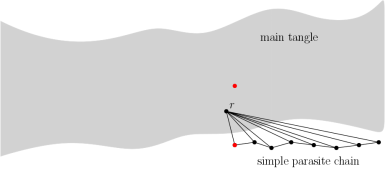
\includegraphics[width=0.45\textwidth]{figures/spc.png}
    \caption{
        An example of simple parasite chain attack, a series of cheat transaction will refer one specific double spent transaction, 
        when the $SPC$ grows to a certain amount, the double spent will be successful, the two red node in the figure respents the 
        conflict transactions.
     }
\label{spc}
\end{center}
\end{figure}


Because the attacker can attack the main network (Main StreamNet) in different forms,
a typical scenario in which we consider the double-spending problem is the Simple Parasite Chain attack.
A simple side chain is shown in Figure~\ref{spc}. 
In \cite{iota_proof}, the author proposed to use local modifier to solve the attack. And in our tip selection algorithm, 
the local modifier is used for filtering malformed tips and the strategy is configurrable. 
Here we discuss one of the local modifier with edge information.
The framework of this algorithm is consistent with the framework of the weight update algorithm in the existing DAG.
The difference is that when making a set join between two approve transactions, a weighted set join is performed, and the weight is determined by edges. 
And the information of the edge is mainly determined by time information. 
For example, in Figure~\ref{edge_info}, assume that each edge is assigned a weight $w1$ to $w12$, 
because transaction $5$ is approved by transactions $6$, $7$, $8$, as a result its weight is $(w1+w2+w3+w6+w1 \cdot w6)$.

The reason for the adding of edge information is that the attacker often sends out a large number of transactions 
within a short period of time to achieve the purpose of rapidly growing the side chain. 
If edge information is used to rescale the weight, the effects of these attacks are attenuated. 
On the contrary, becasue the issuing rate of non-attack type transaction is similar to the speed of the whole network,
and its weight update is similar to the result of the original algorithm.

\begin{figure}[!ht]
\begin{center}
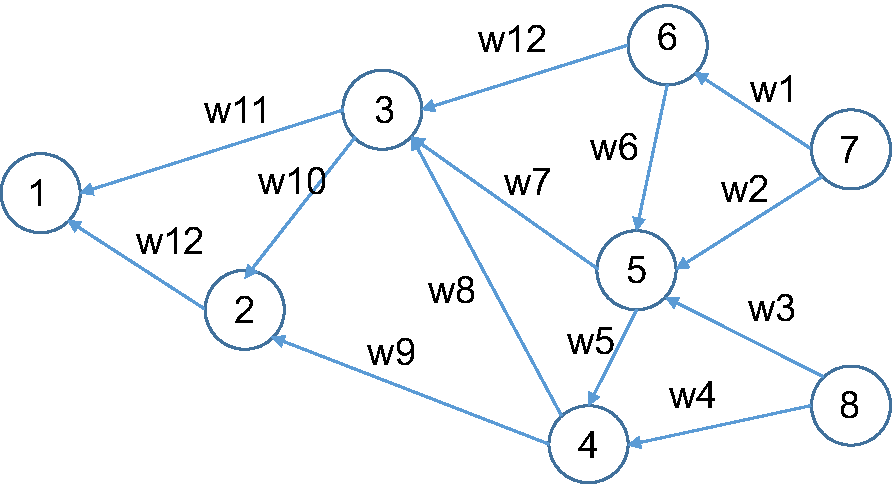
\includegraphics[width=0.40\textwidth]{figures/edge_info.pdf}
    \caption{
        Weight calculation based on edge information.
     }
\label{edge_info}
\end{center}
\end{figure}

